\section{Visualisation des résulats expérimentaux et modèle physique}
\subsection{Visualisations}
\begin{frame}
    \frametitle{Quelques visualisations 1/3}
    \begin{figure}[!h]
        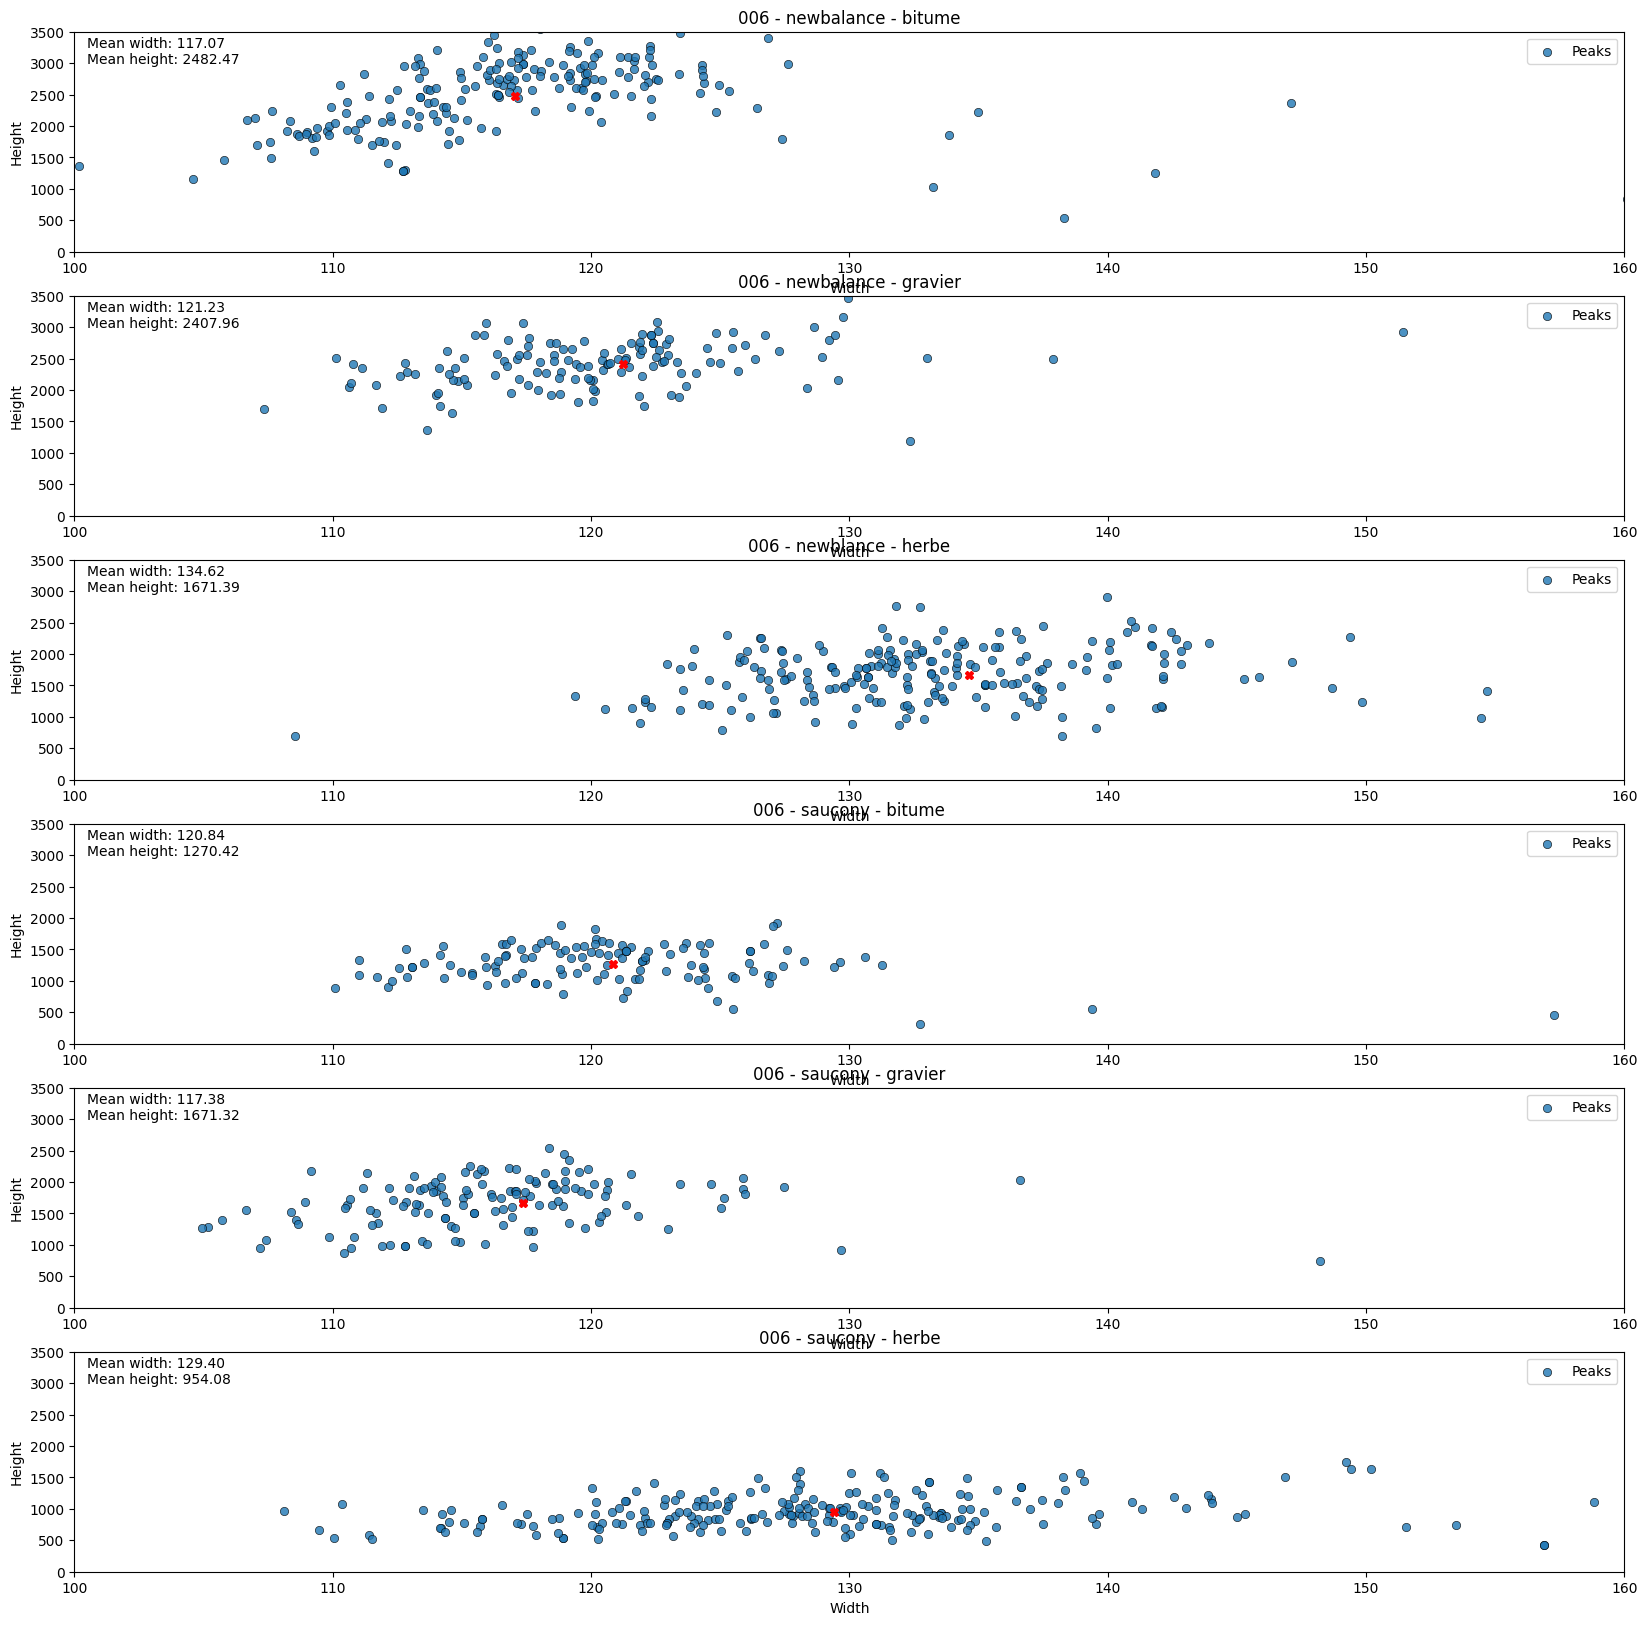
\includegraphics[scale=0.2]{./figures/res_02.png}
    \end{figure}
\end{frame}
\begin{frame}{Quelques visualisations 2/3}
    \begin{figure}
        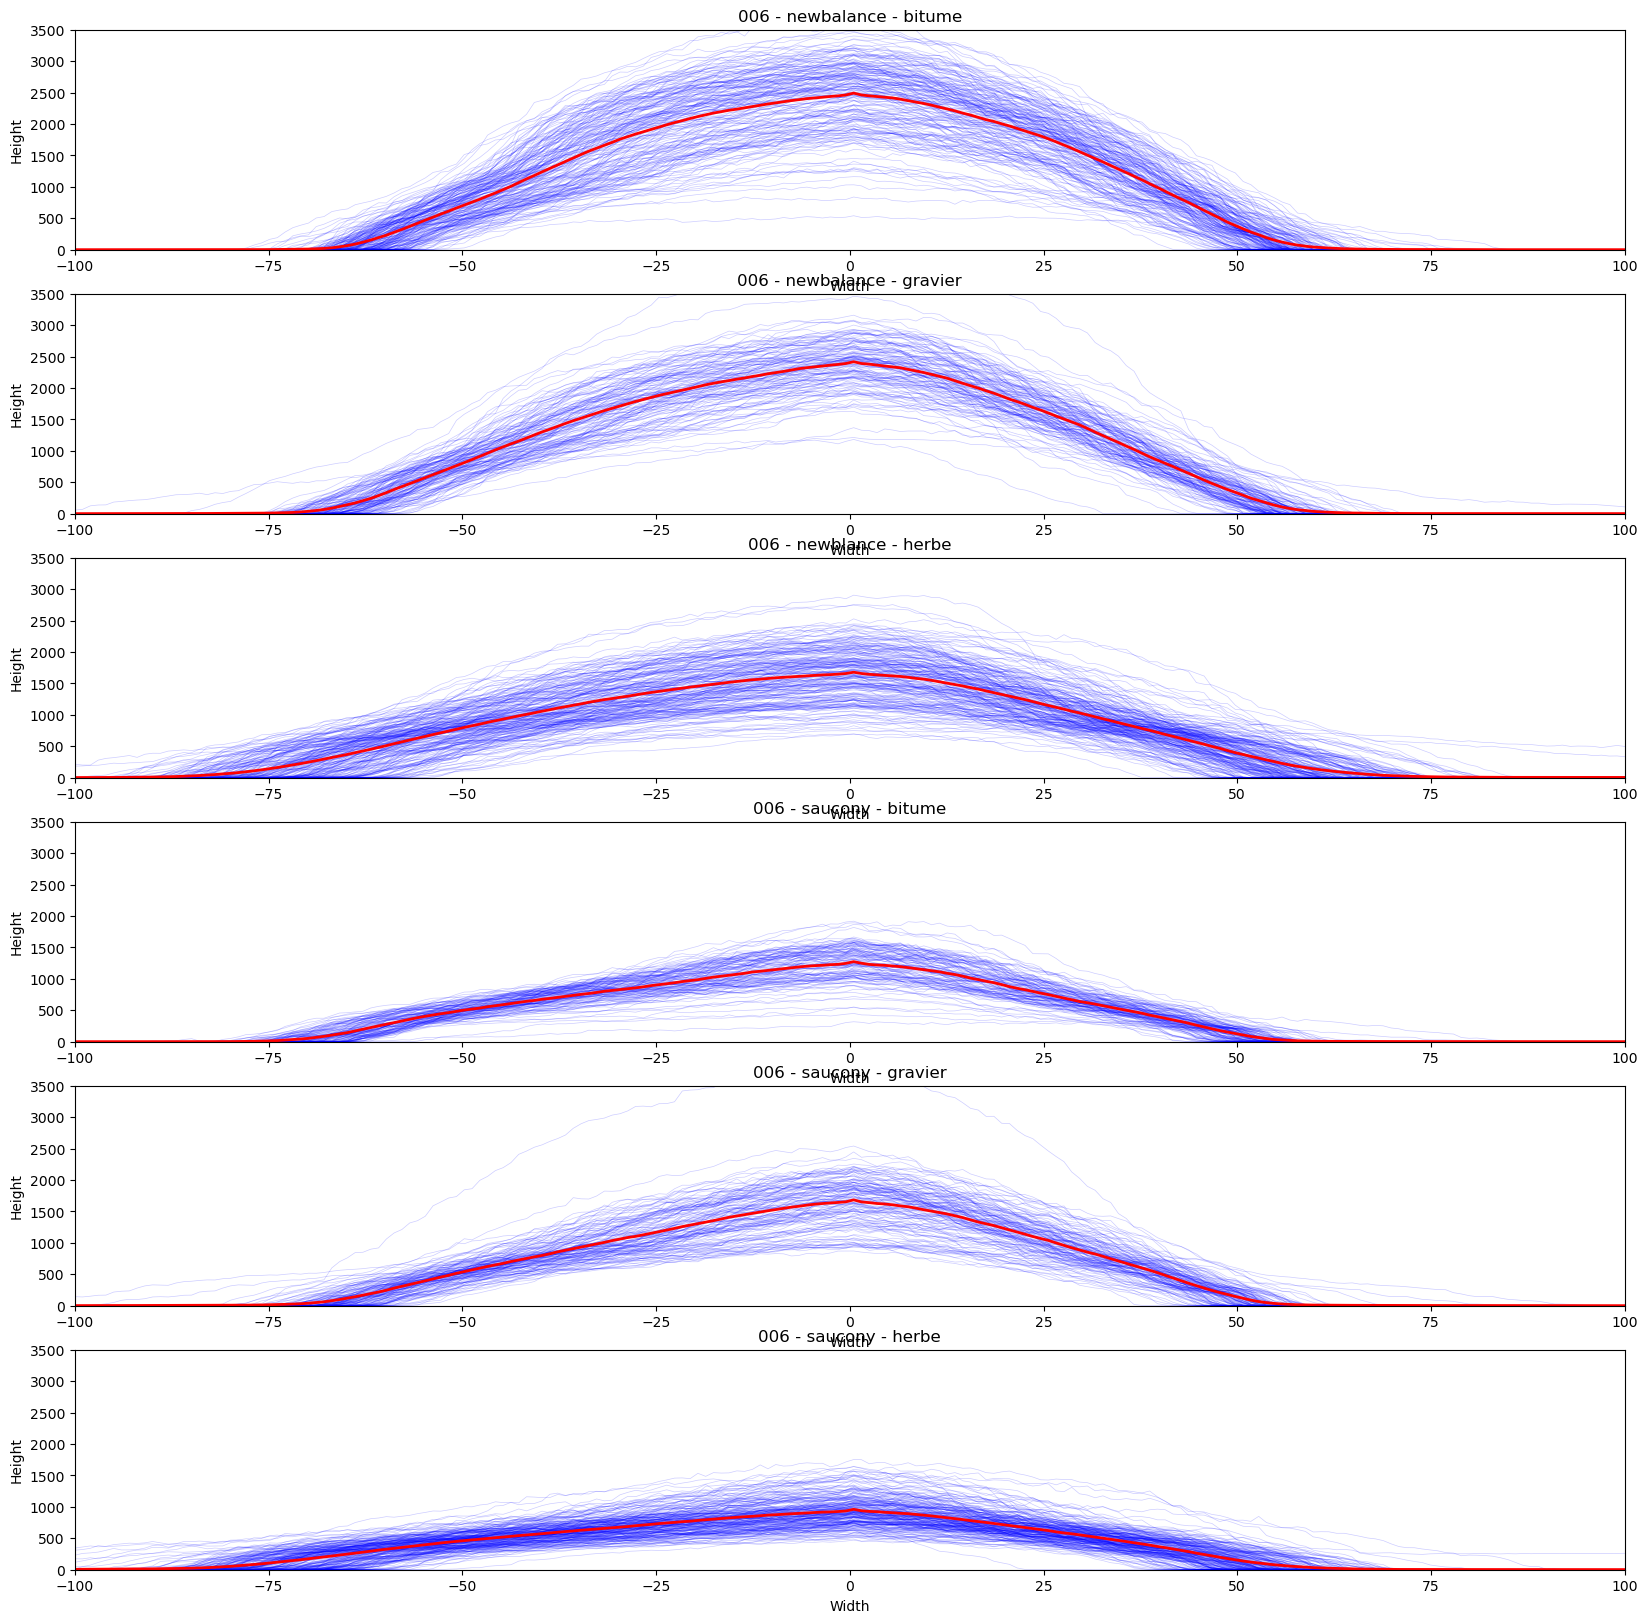
\includegraphics[scale=0.2]{./figures/res_03.png}
    \end{figure}
\end{frame}
\begin{frame}{Quelques visualisations 3/3}
    Gardons ici les pics moyens pour chaque revêtement et type de chaussures:
    \begin{figure}
        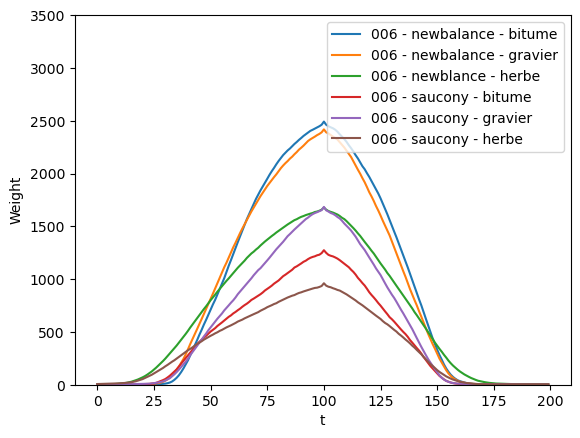
\includegraphics[scale=0.5]{./figures/res_04.png}
    \end{figure}
\end{frame}
\subsection{Modèle physique}
\begin{frame}{Rhéologie}
    L'os est un matériau viscoélastique, utilisons le modèle de Kelvin-Voigt:
    \begin{figure}
        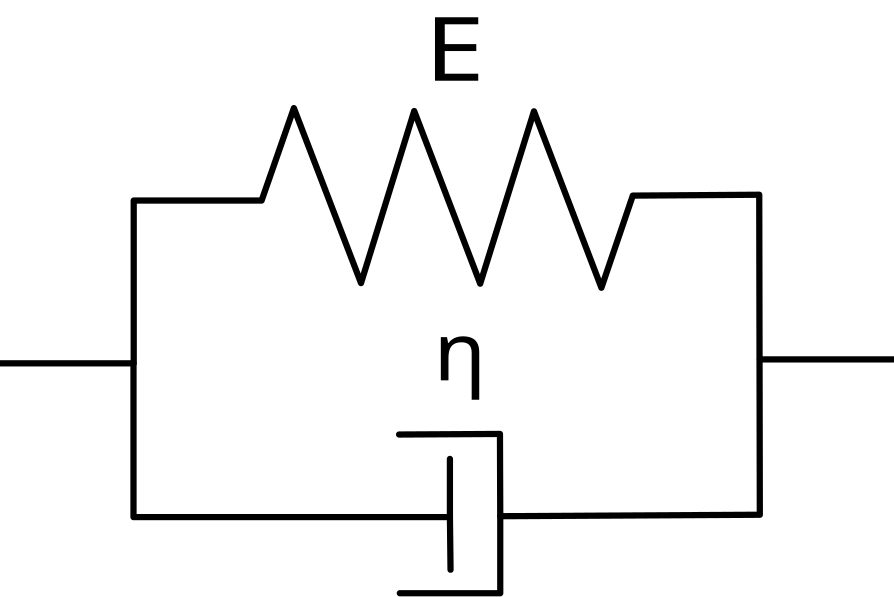
\includegraphics[scale=0.1]{./figures/rheo_00.png}
    \end{figure}
    Nous établissons l'équation différentielle suivante:
    $$ \sigma = E \times \varepsilon + \eta \times \frac{d\varepsilon}{dt}$$
    Et la fonction de transfert associée:
    $$ H(\omega) = \frac{1}{E+i\omega\eta} \quad avec \quad E=18 \cdot 10^9 GPa \quad \eta = 218,4 Pa \cdot sec^{-1}$$
\end{frame}
\begin{frame}{Résultats}
    Puisque $ \omega \ll 10^3 rad \cdot sec^{-1}$, nous avons $ H(\omega) \approx \frac{1}{E}$ on obtient donc:
    \begin{figure}
        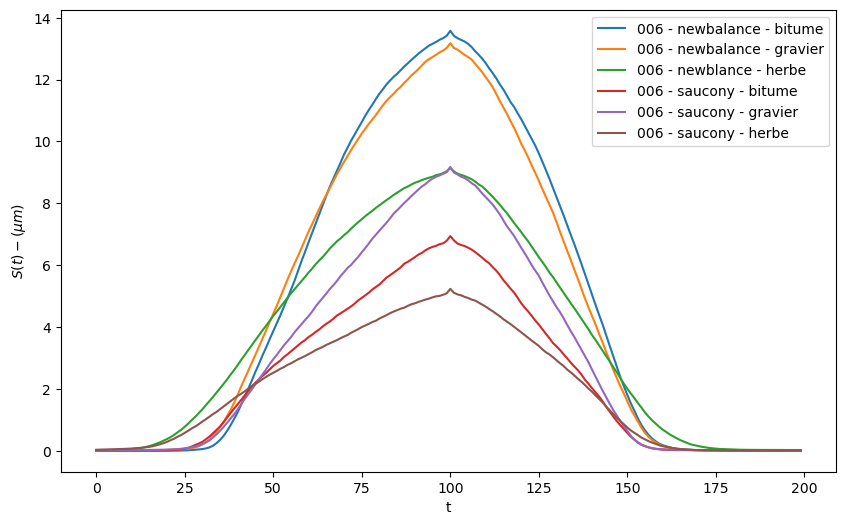
\includegraphics[scale=0.5]{./figures/rheo_05.png}
    \end{figure}
\end{frame}
